% questions.tex —— 2006 年·全国卷Ⅱ·理科 · 题目内容片段（无答案）
% 由 tools/generate_projects.py 依来源总账自 2006/2006_数学真题_全国2理_试题.md 生成，勿手改（改源 MD 后重跑）


\gkpart{数学}

\begin{gktip}
\textbf{来源说明}：本题面依据固定源 PDF 两页 A3 题面逐题转录，原卷印刷页码 316–317。固定源不附答案，答案和解析均由本库独立复算。

\textbf{图形说明}：第 7、16、19、21 题的原卷图形关系重绘为 TikZ/PGFPlots 矢量图。图形标记所指的 PNG 不随仓库保存。
\end{gktip}

\gkpart{一、选择题}

\begin{question}
\gkti{1}设集合 $M=\{x\mid x<3\}$，$N=\{x\mid\log_2x>1\}$，则 $M\cap N=$\mbox{（　　）}

（A）$\varnothing$\quad（B）$\{x\mid0<x<3\}$\quad（C）$\{x\mid1<x<3\}$\quad（D）$\{x\mid2<x<3\}$

\end{question}
\begin{question}
\gkti{2}函数 $y=\sin2x\cos2x$ 的最小正周期是\mbox{（　　）}

（A）$2\pi$\quad（B）$4\pi$\quad（C）$\dfrac\pi4$\quad（D）$\dfrac\pi2$

\end{question}
\begin{question}
\gkti{3}$\dfrac{3}{(1-i)^2}=$\mbox{（　　）}

（A）$\dfrac32i$\quad（B）$-\dfrac32i$\quad（C）$i$\quad（D）$-i$

\end{question}
\begin{question}
\gkti{4}过球的一条半径的中点，作垂直于该半径的平面，则所得截面的面积与球的表面积的比为\mbox{（　　）}

（A）$\dfrac3{16}$\quad（B）$\dfrac9{16}$\quad（C）$\dfrac38$\quad（D）$\dfrac9{32}$

\end{question}
\begin{question}
\gkti{5}已知 $\triangle ABC$ 的顶点 $B,C$ 在椭圆 $\dfrac{x^2}{3}+y^2=1$ 上，顶点 $A$ 是椭圆的一个焦点，且椭圆的另外一个焦点在 $BC$ 边上，则 $\triangle ABC$ 的周长是\mbox{（　　）}

（A）$2\sqrt3$\quad（B）$6$\quad（C）$4\sqrt3$\quad（D）$12$

\end{question}
\begin{question}
\gkti{6}已知函数 $f(x)=\ln x+1\ (x>0)$，则 $f(x)$ 的反函数为\mbox{（　　）}

（A）$y=e^{x+1}\ (x\in\mathbb R)$\quad（B）$y=e^{x-1}\ (x\in\mathbb R)$

（C）$y=e^{x+1}\ (x>1)$\quad（D）$y=e^{x-1}\ (x>1)$

\Needspace{0.4\textheight}
\end{question}
\begin{question}
\gkti{7}如图，平面 $\alpha\perp$ 平面 $\beta$，$A\in\alpha$，$B\in\beta$，$AB$ 与两平面 $\alpha,\beta$ 所成的角分别为 $\dfrac\pi4$ 和 $\dfrac\pi6$。过 $A,B$ 分别作两平面交线的垂线，垂足为 $A',B'$，则 $AB:A'B'=$\mbox{（　　）}
\nopagebreak[4]
\begin{center}% 2006 年全国卷Ⅱ理科第 7 题：两个互相垂直的平面
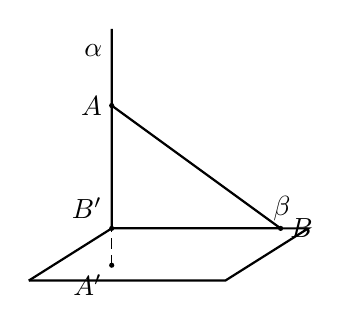
\begin{tikzpicture}[>=stealth,scale=0.78]
  \coordinate (I) at (0,0);
  \coordinate (J) at (1.35,0.85);
  \coordinate (K) at (4.55,0.85);
  \coordinate (L) at (3.20,0);
  \coordinate (Atop) at (1.35,4.10);
  \coordinate (A) at (1.35,2.85);
  \coordinate (Aprime) at (1.35,0.25);
  \coordinate (Bprime) at (1.35,0.85);
  \coordinate (B) at (4.10,0.85);
  \draw[thick] (I)--(J)--(Atop);
  \draw[thick] (I)--(L)--(K)--(J);
  \draw[thick] (J)--(B);
  \draw[thick] (A)--(B);
  \draw[dashed] (A)--(Aprime) (Aprime)--(Bprime);
  \fill (A) circle (1.2pt) node[left] {$A$};
  \fill (Aprime) circle (1.2pt) node[below left] {$A'$};
  \fill (Bprime) circle (1.2pt) node[above left] {$B'$};
  \fill (B) circle (1.2pt) node[right] {$B$};
  \node at (1.05,3.75) {$\alpha$};
  \node at (4.12,1.18) {$\beta$};
\end{tikzpicture}
\end{center}
\nopagebreak[4]
（A）$2:1$\quad（B）$3:1$\quad（C）$3:2$\quad（D）$4:3$

\end{question}
\begin{question}
\gkti{8}已知函数 $y=f(x)$ 的图象与函数 $g(x)=\log_2x\ (x>0)$ 的图象关于原点对称，则 $f(x)$ 的表达式为\mbox{（　　）}

（A）$f(x)=\dfrac1{\log_2x}\ (x>0)$\quad（B）$f(x)=\dfrac1{\log_2(-x)}\ (x<0)$

（C）$f(x)=-\log_2x\ (x>0)$\quad（D）$f(x)=-\log_2(-x)\ (x<0)$

\end{question}
\begin{question}
\gkti{9}已知双曲线 $\dfrac{x^2}{a^2}-\dfrac{y^2}{b^2}=1$ 的一条渐近线方程为 $y=\dfrac43x$，则双曲线的离心率为\mbox{（　　）}

（A）$\dfrac53$\quad（B）$\dfrac43$\quad（C）$\dfrac54$\quad（D）$\dfrac32$

\end{question}
\begin{question}
\gkti{10}若 $f(\sin x)=3-\cos2x$，则 $f(\cos x)=$\mbox{（　　）}

（A）$3-\cos2x$\quad（B）$3-\sin2x$\quad（C）$3+\cos2x$\quad（D）$3+\sin2x$

\end{question}
\begin{question}
\gkti{11}设 $S_n$ 是等差数列 $\{a_n\}$ 的前 $n$ 项和，若 $\dfrac{S_3}{S_6}=\dfrac13$，则 $\dfrac{S_6}{S_{12}}=$\mbox{（　　）}

（A）$\dfrac3{10}$\quad（B）$\dfrac13$\quad（C）$\dfrac18$\quad（D）$\dfrac19$

\end{question}
\begin{question}
\gkti{12}函数 $\displaystyle\sum_{n=1}^{19}|x-n|$ 的最小值为\mbox{（　　）}

（A）$190$\quad（B）$171$\quad（C）$90$\quad（D）$45$

\end{question}
\gkpart{二、填空题}

\begin{question}
\gkti{13}在 $\left(x^4+\dfrac1x\right)^{10}$ 的展开式中常数项是\gkblank{}。（用数字作答）

\end{question}
\begin{question}
\gkti{14}已知 $\triangle ABC$ 的三个内角 $A,B,C$ 成等差数列，且 $AB=1,BC=4$，则边 $BC$ 上的中线 $AD$ 的长为\gkblank{}。

\end{question}
\begin{question}
\gkti{15}过点 $(1,\sqrt2)$ 的直线 $l$ 将圆 $(x-2)^2+y^2=4$ 分成两段弧，当劣弧所对的圆心角最小时，直线 $l$ 的斜率 $k=$\gkblank{}。

\Needspace{0.4\textheight}
\end{question}
\begin{question}
\gkti{16}一个社会调查机构就某地居民的月收入调查了 $10000$ 人，并根据所得数据画了样本的频率分布直方图（如图）。为了分析居民的收入与年龄、学历、职业等方面的关系，要从这 $10000$ 人中再用分层抽样方法抽出 $100$ 人作进一步调查，则在 $[2500,3000)$（元）月收入段应抽出\gkblank{}人。
\nopagebreak[4]
\begin{center}% 2006 年全国卷Ⅱ理科第 16 题：月收入频率分布直方图
\begin{tikzpicture}[>=stealth,scale=0.72]
  \draw[->] (0,0)--(8.4,0) node[right] {月收入（元）};
  \draw[->] (0,0)--(0,3.45) node[above] {频率\(/\)组距};
  \foreach \y/\lab in {0.65/0.0001,1.30/0.0002,1.95/0.0003,2.60/0.0004,3.25/0.0005} {
    \draw[dashed,gray] (0,\y)--(7.65,\y);
    \node[left] at (0,\y) {\scriptsize\lab};
  }
  \draw (1,0) rectangle (2,1.30);
  \draw (2,0) rectangle (3,2.60);
  \draw (3,0) rectangle (4,3.25);
  \draw (4,0) rectangle (5,3.25);
  \draw (5,0) rectangle (6,1.95);
  \draw (6,0) rectangle (7,0.65);
  \foreach \x/\lab in {0/0,1/1000,2/1500,3/2000,4/2500,5/3000,6/3500,7/4000} {
    \node[below] at (\x,0) {\scriptsize\lab};
  }
  \draw[thick] (0.95,0.08)--(1.05,-0.08)--(1.15,0.08);
\end{tikzpicture}
\end{center}
\nopagebreak[4]
\end{question}
\gkpart{三、解答题}

\begin{question}
\gkti{17}已知向量 $\boldsymbol a=(\sin\theta,\sqrt3)$，$\boldsymbol b=(1,\cos\theta)$，$-\dfrac\pi2<\theta<\dfrac\pi2$。

（1） 若 $\boldsymbol a\perp\boldsymbol b$，求 $\theta$；

（2） 求 $|\boldsymbol a+\boldsymbol b|$ 的最大值。

\end{question}
\begin{question}
\gkti{18}某批产品成箱包装，每箱 $5$ 件。一用户在购进该批产品前先取出 $3$ 箱，再从每箱中任意取出 $2$ 件产品进行检验。设取出的第一、二、三箱中分别有 $0$ 件、$1$ 件、$2$ 件二等品，其余为一等品。

（1） 用 $\xi$ 表示抽检的 $6$ 件产品中二等品的件数，求 $\xi$ 的分布列及 $\xi$ 的数学期望；

（2） 若抽检的 $6$ 件产品中有 $2$ 件或 $2$ 件以上二等品，用户就拒绝购买这批产品，求这批产品被用户拒绝购买的概率。

\Needspace{0.4\textheight}
\end{question}
\begin{question}
\gkti{19}如图，在直三棱柱 $ABC-A_1B_1C_1$ 中，$AB=BC$，$D,E$ 分别为 $BB_1,AC_1$ 的中点。
\nopagebreak[4]
\begin{center}% 2006 年全国卷Ⅱ理科第 19 题：直三棱柱
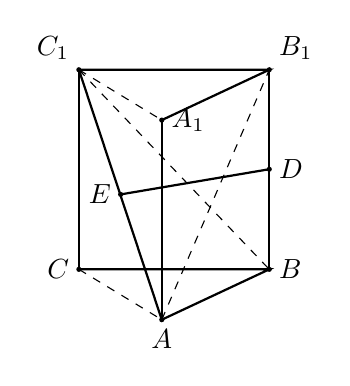
\begin{tikzpicture}[>=stealth,scale=0.78]
  \coordinate (A) at (2.20,0);
  \coordinate (B) at (3.95,0.82);
  \coordinate (C) at (0.85,0.82);
  \coordinate (A1) at (2.20,3.25);
  \coordinate (B1) at (3.95,4.07);
  \coordinate (C1) at (0.85,4.07);
  \coordinate (D) at (3.95,2.45);
  \coordinate (E) at (1.53,2.04);
  \draw[thick] (A)--(B)--(C);
  \draw[dashed] (C)--(A);
  \draw[thick] (A)--(A1) (B)--(B1) (C)--(C1);
  \draw[thick] (A1)--(B1)--(C1);
  \draw[dashed] (C1)--(A1);
  \draw[thick] (A)--(C1);
  \draw[dashed] (B)--(B1) (A)--(B1) (C1)--(B);
  \draw[thick] (D)--(E);
  \fill (A) circle (1.2pt) node[below] {$A$};
  \fill (B) circle (1.2pt) node[right] {$B$};
  \fill (C) circle (1.2pt) node[left] {$C$};
  \fill (A1) circle (1.2pt) node[right] {$A_1$};
  \fill (B1) circle (1.2pt) node[above right] {$B_1$};
  \fill (C1) circle (1.2pt) node[above left] {$C_1$};
  \fill (D) circle (1.2pt) node[right] {$D$};
  \fill (E) circle (1.2pt) node[left] {$E$};
\end{tikzpicture}
\end{center}
\nopagebreak[4]
（1） 证明：$ED$ 为异面直线 $BB_1$ 与 $AC_1$ 的公垂线；

（2） 设 $AA_1=AC=\sqrt2AB$，求二面角 $A_1-AD-C_1$ 的大小。

\end{question}
\begin{question}
\gkti{20}设函数 $f(x)=(x+1)\ln(x+1)$。若对所有的 $x\geqslant0$，都有 $f(x)\geqslant ax$ 成立，求实数 $a$ 的取值范围。

\Needspace{0.4\textheight}
\end{question}
\begin{question}
\gkti{21}已知抛物线 $x^2=4y$ 的焦点为 $F$，$A\text{、}B$ 是抛物线上的两动点，且 $\overrightarrow{AF}=\lambda\overrightarrow{FB}\ (\lambda>0)$。过 $A,B$ 两点分别作抛物线的切线，设其交点为 $M$。
\nopagebreak[4]
\begin{center}% 2006 年全国卷Ⅱ理科第 21 题：抛物线与两条切线
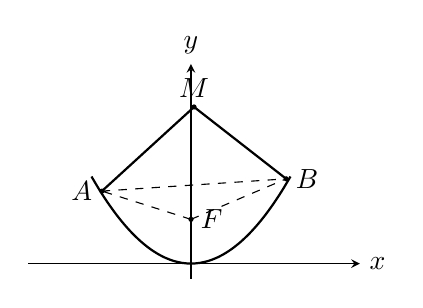
\begin{tikzpicture}[>=stealth,scale=0.78]
  \draw[->] (-2.65,0)--(2.75,0) node[right] {$x$};
  \draw[->] (0,-0.25)--(0,3.25) node[above] {$y$};
  \draw[thick] plot[smooth,domain=-2.25:2.25] ({0.72*\x},{0.28*\x*\x});
  \coordinate (F) at (0,0.72);
  \coordinate (A) at (-1.45,1.18);
  \coordinate (B) at (1.55,1.38);
  \coordinate (M) at (0.05,2.55);
  \draw[dashed] (A)--(B) (F)--(A) (F)--(B);
  \draw[thick] (A)--(M) (B)--(M);
  \fill (F) circle (1.2pt) node[right] {$F$};
  \fill (A) circle (1.2pt) node[left] {$A$};
  \fill (B) circle (1.2pt) node[right] {$B$};
  \fill (M) circle (1.2pt) node[above] {$M$};
\end{tikzpicture}
\end{center}
\nopagebreak[4]
（1） 证明 $\overrightarrow{FM}\cdot\overrightarrow{AB}$ 为定值；

（2） 设 $\triangle ABM$ 的面积为 $S$，写出 $S=f(\lambda)$ 的表达式，并求 $S$ 的最小值。

\end{question}
\begin{question}
\gkti{22}设数列 $\{a_n\}$ 的前 $n$ 项和为 $S_n$，且方程 $x^2-a_nx-a_n=0$ 有一根为 $S_n-1$，$n=1,2,3,\ldots$。

（1） 求 $a_1,a_2$；

（2） 求 $\{a_n\}$ 的通项公式。

\end{question}